\documentclass[11pt,a4paper]{article}
\usepackage[top=3cm,bottom=3cm,left=4cm,right=3cm]{geometry}
\usepackage[T1]{fontenc}
\usepackage{lmodern}
\usepackage{microtype}
\usepackage{amsmath}
\usepackage{amssymb}
\usepackage[htt]{hyphenat}
\usepackage{xurl}
\usepackage{graphicx}
\usepackage{caption}
\usepackage{float}
\usepackage{array}
\usepackage{tabularx}
\usepackage{enumitem}
\usepackage{xcolor}
\usepackage{tikz}
\usepackage{pgfplots}
\usetikzlibrary{calc,positioning}
\usepackage{multirow}
\pgfplotsset{compat=1.16}
\usepackage{listings}
\usepackage{fancyhdr}
\usepackage[colorlinks=true,linkcolor=blue,urlcolor=blue]{hyperref}

% Istilah dalam Bahasa Indonesia (tanpa babel agar kompatibel di semua TeX)
\renewcommand{\contentsname}{Daftar Isi}
\renewcommand{\figurename}{Gambar}
\renewcommand{\tablename}{Tabel}
\renewcommand{\lstlistingname}{Kode}
\renewcommand{\appendixname}{Lampiran}
\renewcommand{\refname}{Daftar Pustaka}

% Header dan footer
\pagestyle{fancy}
\fancyhf{}
\fancyhead[L]{Modul 2 -- Kontrol Kecepatan}
\fancyhead[R]{\nouppercase{\leftmark}}
\fancyfoot[L]{TF4015 Sistem Kontrol Diskrit}
\fancyfoot[R]{\thepage}
\renewcommand{\footrulewidth}{0.4pt}
\setlength{\headheight}{14pt}

% Gaya penulisan kode
\lstset{
language=C++,
basicstyle=\ttfamily\footnotesize,
keywordstyle=\color{blue!70!black}\bfseries,
commentstyle=\color{green!45!black},
stringstyle=\color{red!65!black},
numbers=left,
numberstyle=\tiny\color{gray},
frame=single,
breaklines=true,
tabsize=2,
showstringspaces=false,
columns=fullflexible,
keepspaces=true,
morekeywords={byte,uint32_t,String}
}

% Makro bantu
% Nama sketch utama program praktikum. Ubah di sini bila nama di repositori berbeda.
\newcommand{\sketch}{\texttt{SKD23.ino}}
% Nama file/program dalam teks
\newcommand{\prog}[1]{\texttt{#1}}
% Gambar dengan placeholder: bila file belum ada, ditampilkan kotak penanda
\newcommand{\gambar}[4]{%
\begin{figure}[H]
\centering
\IfFileExists{#1}{%
\includegraphics[width=#2]{#1}%
}{%
\fbox{\parbox[c][4cm][c]{0.7\textwidth}{\centering\small\textcolor{red}{Gambar belum tersedia:}\\\texttt{\detokenize{#1}}}}%
}
\caption{#3}
\label{#4}
\end{figure}}
% Kotak catatan / peringatan
\newcommand{\peringatan}[1]{%
\begin{center}
\fcolorbox{red!70!black}{red!5}{\parbox{0.92\textwidth}{\textbf{Peringatan.} #1}}
\end{center}}
\newcommand{\catatan}[1]{%
\begin{center}
\fcolorbox{blue!60!black}{blue!4}{\parbox{0.92\textwidth}{\textbf{Catatan.} #1}}
\end{center}}

\renewcommand{\arraystretch}{1.2}
\newcolumntype{C}{>{\centering\arraybackslash}X}
\setlength{\emergencystretch}{3em}
\setlist[itemize]{itemsep=2pt,topsep=4pt}
\setlist[enumerate]{itemsep=2pt,topsep=4pt}

\begin{document}

% Halaman judul
\begin{titlepage}
\centering
\vspace*{2cm}
{\large TF4015 -- Sistem Kontrol Diskrit\par}
\vspace{2.5cm}
{\Large Praktikum\par}
\vspace{0.4cm}
{\huge\bfseries Modul 2\par}
\vspace{0.4cm}
{\LARGE Kontrol Kecepatan\\Motor DC\par}
\vfill
% TODO: sesuaikan nama tim pengajar dan asisten
{\large Tim Pengajar TF4015\par}
\vspace{0.3cm}
{\large Program Studi Teknik Fisika\\Fakultas Teknologi Industri\\Institut Teknologi Bandung\par}
\vspace{0.8cm}
{\large Semester I 2026/2027\par}
\end{titlepage}

\pagenumbering{roman}
\tableofcontents
\newpage
\pagenumbering{arabic}
\setcounter{page}{1}

\section{Pendahuluan}
\subsection{Latar Belakang}
Pengendalian kecepatan putar motor merupakan kasus inti pada berbagai aplikasi, seperti elevator, ban berjalan, dan pompa. Pada Modul 1, kecepatan motor DC telah dimodelkan sebagai sistem orde satu dengan waktu tunda (FOPDT), \textit{deadzone} telah dikompensasi, dan waktu cacah telah ditentukan. Dengan bekal tersebut, pada Modul 2 sistem dikendalikan secara \textbf{kalang tertutup}.

Parameter pengontrol PID dihitung dari model FOPDT menggunakan metode empirik Ziegler--Nichols dan Cohen--Coon, lalu disimulasikan sebelum diterapkan pada kit. Pengontrol diimplementasikan sebagai PID diskrit pada Arduino, lengkap dengan pembatas keluaran dan \textit{anti-windup}. Performa hasil simulasi dan implementasi dibandingkan, kemudian ditingkatkan melalui penalaan halus. Praktikan juga mengamati pengaruh waktu cacah terhadap performa pengontrolan.

\subsection{Tujuan Praktikum}
Setelah menyelesaikan Modul 2, praktikan diharapkan mampu:
\begin{enumerate}
\item Menghitung parameter pengontrol P, PI, dan PID dengan metode Ziegler--Nichols dan Cohen--Coon, lalu menyimulasikannya.
\item Mengimplementasikan pengontrol PID diskrit dengan pembatas keluaran dan \textit{anti-windup} pada kit praktikum.
\item Menilai performa pengontrolan secara kualitatif dan kuantitatif.
\item Meningkatkan performa pengontrolan melalui penalaan halus.
\item Menganalisis pengaruh waktu cacah terhadap performa pengontrolan.
\end{enumerate}

\subsection{Peralatan dan Perangkat Lunak}
\begin{table}[H]
\centering
\caption{Daftar peralatan praktikum Modul 2}
\label{tab:peralatan}
\begin{tabularx}{\textwidth}{|c|X|l|}
\hline
\textbf{No} & \textbf{Nama Peralatan} & \textbf{Keterangan} \\
\hline
1 & Kit praktikum SKD (kit yang sama dengan Modul 0 dan 1) & Disediakan asisten \\
2 & Laptop dengan Arduino IDE dan \textit{library} Adafruit MCP4725 & Milik praktikan \\
3 & MATLAB (desktop atau MATLAB Online) & Milik praktikan \\
4 & Perangkat lunak \textit{spreadsheet} & Milik praktikan \\
5 & Program: \prog{5\_control.ino} (versi Modul 2), \prog{8\_main\_kontrol\_kecepatan} & Unduh dari repositori \\
6 & Skrip MATLAB \prog{simulasi\_kontrol\_kecepatan.m} dan \prog{identifikasi\_fopdt.m} & Unduh dari repositori \\
7 & Model final dan kompensasi \textit{deadzone} dari Modul 1 & Hasil praktikum sebelumnya \\
\hline
\end{tabularx}
\end{table}

\subsection{Persiapan Praktikum}
\begin{enumerate}
\item Siapkan model final Modul 1 ($K$, $\tau$, $\theta$, $T_{s1}$, $T_{s2}$, kecepatan maksimum) dan nilai \texttt{DeadZonePositif} serta \texttt{DeadZoneNegatif} yang digunakan.
\item Ganti tab \prog{5\_control.ino} dengan versi Modul 2 (Kode~\ref{lst:control}) dan pahami setiap barisnya.
\item Jalankan skrip \prog{simulasi\_kontrol\_kecepatan.m} dengan model kelompok. Hasil simulasi sebaiknya sudah tersedia sebelum praktikum.
\item Baca prosedur dan bagian analisis, lalu bagi tugas dalam kelompok.
\end{enumerate}

\section{Teori Dasar}
\subsection{Sistem Kontrol Kecepatan Kalang Tertutup}
Struktur sistem kontrol kecepatan pada kit praktikum ditunjukkan pada Gambar~\ref{fig:diagram_blok}. Set point kecepatan $r$ dibandingkan dengan kecepatan terukur $y$ untuk menghasilkan error $e = r - y$. Pengontrol PID menghitung aksi kontrol $u$ yang kemudian dibatasi, dikompensasi \textit{deadzone}-nya, dan diberikan kepada driver motor. Kecepatan motor diukur oleh tachometer melalui rangkaian pengkondisi sinyal dan ADC. Seluruh perhitungan dilakukan setiap waktu cacah $T_s$.

\begin{figure}[H]
\centering
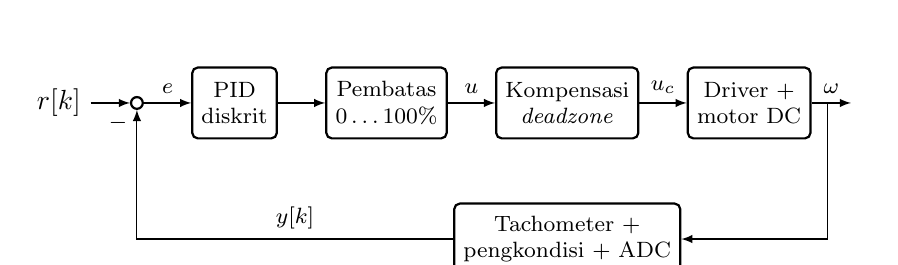
\begin{tikzpicture}[
blok/.style={draw, thick, rounded corners=2pt, minimum height=9mm, align=center, font=\footnotesize},
jum/.style={draw, thick, circle, inner sep=1.5pt},
>=latex, node distance=6mm]
\node (r) {$r[k]$};
\node[jum, right=5mm of r] (s) {};
\node[blok, right=of s] (pid) {PID\\diskrit};
\node[blok, right=of pid] (sat) {Pembatas\\$0 \ldots 100\%$};
\node[blok, right=of sat] (komp) {Kompensasi\\\textit{deadzone}};
\node[blok, right=of komp] (plant) {Driver +\\motor DC};
\node[blok, below=8mm of komp] (sens) {Tachometer +\\pengkondisi + ADC};
\node[right=5mm of plant] (y) {};
\draw[->] (r) -- (s);
\draw[->] (s) -- node[above, font=\footnotesize] {$e$} (pid);
\draw[->] (pid) -- (sat);
\draw[->] (sat) -- node[above, font=\footnotesize] {$u$} (komp);
\draw[->] (komp) -- node[above, font=\footnotesize] {$u_c$} (plant);
\draw[->] (plant) -- node[above, font=\footnotesize] {$\omega$} (y);
\draw[->] ($(plant.east)+(2mm,0)$) |- (sens);
\draw[->] (sens) -| node[pos=0.95, left, font=\footnotesize] {$-$} node[pos=0.25, above, font=\footnotesize] {$y[k]$} (s);
\end{tikzpicture}
\caption{Diagram blok sistem kontrol kecepatan pada kit praktikum}
\label{fig:diagram_blok}
\end{figure}

Model yang digunakan untuk perancangan adalah model FOPDT dari Modul 1, yaitu hubungan antara masukan sebelum kompensasi $u$ dan kecepatan terukur $y$:
\begin{equation}
G(s) = \frac{K\,e^{-\theta s}}{\tau s + 1}.
\label{eq:fopdt}
\end{equation}
Karena tachometer hanya membaca besar kecepatan, kontrol kecepatan pada modul ini dibatasi untuk satu arah putar, dan keluaran pengontrol dibatasi pada $0 \le u \le 100\%$.

\subsection{Pengontrol PID Kontinu dan Diskrit}
Pengontrol PID kontinu dinyatakan sebagai
\begin{equation}
u(t) = K_p\left(e(t) + \frac{1}{T_i}\int_0^t e(\lambda)\,d\lambda + T_d\,\frac{de(t)}{dt}\right)
= K_p\,e(t) + K_i\int_0^t e(\lambda)\,d\lambda + K_d\,\frac{de(t)}{dt},
\label{eq:pid}
\end{equation}
dengan $K_i = K_p/T_i$ dan $K_d = K_p T_d$. Pada mikrokontroler, integral didekati dengan penjumlahan persegi panjang dan turunan didekati dengan selisih mundur, sehingga diperoleh PID diskrit bentuk posisi
\begin{equation}
u[k] = K_p\,e[k] + K_i\,T_s\sum_{i=0}^{k} e[i] + K_d\,\frac{e[k] - e[k-1]}{T_s}.
\label{eq:pid_diskrit}
\end{equation}
Pada tab \prog{5\_control.ino}, waktu dinyatakan dalam milidetik, sehingga $K_i$ bersatuan 1/ms dan $K_d$ bersatuan ms. Dengan cara ini, nilai $K_p$, $K_i$, dan $K_d$ \textbf{tidak bergantung pada waktu cacah}; waktu cacah hanya memengaruhi seberapa baik persamaan~\eqref{eq:pid_diskrit} mendekati persamaan~\eqref{eq:pid}.

Selain itu, pencacahan dengan \textit{zero-order hold} menambah keterlambatan efektif sekitar setengah waktu cacah. Sistem yang dikontrol secara diskrit berperilaku kurang lebih seperti sistem kontinu dengan waktu tunda
\begin{equation}
\theta_{\text{efektif}} \approx \theta + \frac{T_s}{2}.
\label{eq:theta_efektif}
\end{equation}
Semakin besar $T_s$, semakin besar waktu tunda efektif, sehingga margin kestabilan berkurang.

\subsection{Saturasi dan \textit{Anti-Windup}}
Aksi kontrol pada kit dibatasi pada $0$--$100\%$. Ketika keluaran saturasi, misalnya saat set point berubah besar, error tetap diakumulasi oleh bagian integral sehingga nilainya membesar jauh melebihi yang dibutuhkan (\textit{integrator windup}). Akibatnya, setelah keluaran mencapai set point, integral memerlukan waktu lama untuk turun dan menyebabkan \textit{overshoot} besar. Tab \prog{5\_control.ino} menggunakan \textbf{integrasi bersyarat}: error hanya diakumulasi bila keluaran tidak saturasi, atau bila tanda error membantu keluaran keluar dari saturasi.

\subsection{Penalaan Ziegler--Nichols dan Cohen--Coon}
Untuk model FOPDT, parameter awal pengontrol dapat dihitung dengan rumus empirik pada Tabel~\ref{tab:rumus_penalaan} \cite{seborg}. Metode Ziegler--Nichols kurva reaksi umumnya menghasilkan respons dengan rasio peluruhan seperempat, sedangkan Cohen--Coon memperhitungkan rasio $r = \theta/\tau$ secara lebih eksplisit.

\begin{table}[H]
\centering
\caption{Rumus penalaan untuk model FOPDT ($r = \theta/\tau$)}
\label{tab:rumus_penalaan}
\renewcommand{\arraystretch}{2.1}
\begin{tabular}{|c|c|c|c|}
\hline
\textbf{Metode} & \textbf{Kontrol} & $K_p$ & $T_i$, $T_d$ \\
\hline
\multirow{3}{*}{Ziegler--Nichols} & P & $\dfrac{\tau}{K\theta}$ & -- \\
\cline{2-4}
& PI & $\dfrac{0{,}9\,\tau}{K\theta}$ & $T_i = 3{,}33\,\theta$ \\
\cline{2-4}
& PID & $\dfrac{1{,}2\,\tau}{K\theta}$ & $T_i = 2\theta$, $T_d = 0{,}5\theta$ \\
\hline
\multirow{3}{*}{Cohen--Coon} & P & $\dfrac{\tau}{K\theta}\left(1 + \dfrac{r}{3}\right)$ & -- \\
\cline{2-4}
& PI & $\dfrac{\tau}{K\theta}\left(0{,}9 + \dfrac{r}{12}\right)$ & $T_i = \theta\,\dfrac{30 + 3r}{9 + 20r}$ \\
\cline{2-4}
& PID & $\dfrac{\tau}{K\theta}\left(\dfrac{4}{3} + \dfrac{r}{4}\right)$ & $T_i = \theta\,\dfrac{32 + 6r}{13 + 8r}$, $T_d = \dfrac{4\theta}{11 + 2r}$ \\
\hline
\end{tabular}
\end{table}

\subsection{Parameter Performa Pengontrolan}
Performa respons terhadap perubahan set point dinilai dengan parameter berikut (Gambar~\ref{fig:performa}):
\begin{itemize}
\item \textbf{\textit{Delay time}} $t_d$: waktu hingga respons mencapai 50\% nilai akhir.
\item \textbf{\textit{Rise time}} $t_r$: waktu yang diperlukan respons untuk naik dari 10\% hingga 90\% nilai akhir.
\item \textbf{\textit{Overshoot}} $M_p$: selisih nilai puncak terhadap nilai akhir, dalam persen nilai akhir.
\item \textbf{\textit{Settling time}} $t_s$: waktu hingga respons tetap berada dalam pita $\pm 2\%$ nilai akhir.
\item \textbf{\textit{Offset}} $e_{ss}$: selisih set point dengan nilai akhir respons.
\end{itemize}
Semua waktu dihitung sejak set point berubah. Untuk pengontrol P pada sistem FOPDT, nilai akhir tidak sama dengan set point; offset teoretisnya adalah
\begin{equation}
e_{ss} = \frac{r}{1 + K K_p}.
\label{eq:offset}
\end{equation}

\begin{figure}[H]
\centering
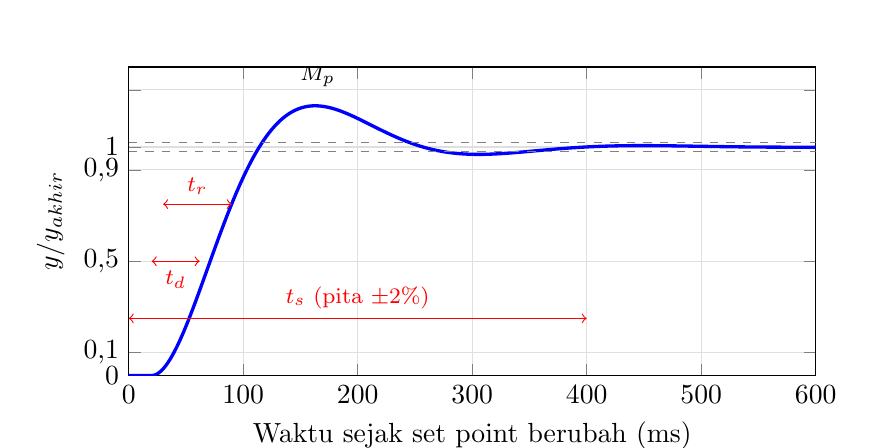
\begin{tikzpicture}
\begin{axis}[width=0.85\textwidth, height=5.5cm, xmin=0, xmax=600, ymin=0, ymax=1.35,
xlabel={Waktu sejak set point berubah (ms)}, ylabel={$y / y_{akhir}$},
grid=major, grid style={gray!25}, ytick={0,0.1,0.5,0.9,1,1.25}, yticklabels={0,{0,1},{0,5},{0,9},1,{}}]
\addplot[very thick, blue, domain=0:600, samples=300] {x<20 ? 0 : 1-exp(-0.012*(x-20))*(cos(deg(0.022*(x-20))) + 0.5454*sin(deg(0.022*(x-20))))};
\addplot[dashed, gray] coordinates {(0,1.02) (600,1.02)};
\addplot[dashed, gray] coordinates {(0,0.98) (600,0.98)};
\node[font=\footnotesize, anchor=south] at (axis cs:165,1.22) {$M_p$};
\draw[<->, red] (axis cs:20,0.5) -- (axis cs:62,0.5) node[midway, below, font=\footnotesize] {$t_d$};
\draw[<->, red] (axis cs:30,0.75) -- (axis cs:90,0.75) node[midway, above, font=\footnotesize] {$t_r$};
\draw[<->, red] (axis cs:0,0.25) -- (axis cs:400,0.25) node[midway, above, font=\footnotesize] {$t_s$ (pita $\pm2\%$)};
\end{axis}
\end{tikzpicture}
\caption{Ilustrasi parameter performa respons terhadap perubahan set point}
\label{fig:performa}
\end{figure}

Pengaruh umum setiap parameter terhadap respons kalang tertutup dirangkum pada Tabel~\ref{tab:pengaruh}. Tabel ini menjadi panduan kualitatif pada penalaan halus; pengaruh sebenarnya dapat berbeda karena saling bergantung.

\begin{table}[H]
\centering
\caption{Pengaruh umum kenaikan parameter PID}
\label{tab:pengaruh}
\begin{tabularx}{\textwidth}{|c|C|C|C|C|}
\hline
\textbf{Parameter naik} & \textbf{\textit{Rise time}} & \textbf{\textit{Overshoot}} & \textbf{\textit{Settling time}} & \textbf{Offset} \\
\hline
$K_p$ & turun & naik & sedikit berubah & turun \\
$K_i$ & turun & naik & naik & hilang \\
$K_d$ & sedikit berubah & turun & turun & tidak berubah \\
\hline
\end{tabularx}
\end{table}

\section{Keselamatan Kerja}
Seluruh ketentuan keselamatan kerja dan SOP pada Modul 0 tetap berlaku. Perhatikan pula hal-hal berikut:
\begin{enumerate}
\item Verifikasi setiap perubahan program tanpa daya motor. Pastikan kolom \texttt{MV} tidak pernah negatif dan tidak melebihi 100.
\item Bila motor berosilasi keras atau kecepatan tidak terkendali, segera cabut kabel listrik 220~V, lalu turunkan $K_p$ atau $K_d$.
\item Jangan mengubah trimpot penguatan OpAmp maupun nilai kompensasi \textit{deadzone}, karena model Modul 1 bergantung pada keduanya.
\end{enumerate}

\section{Prosedur Praktikum}
Prosedur Modul 2 terdiri atas empat percobaan. Percobaan~1 dikerjakan di MATLAB dan dapat dilakukan secara paralel dengan persiapan program pada Percobaan~2. Simpan seluruh data mentah dari \textit{Serial Monitor} ke file teks.

\subsection{Percobaan 1: Parameter Kontrol dan Simulasi}
\begin{enumerate}
\item Lengkapi Tabel~\ref{tab:p1_model} dengan model final dari Modul 1.
\item Isi parameter model pada skrip \prog{simulasi\_kontrol\_kecepatan.m} (Kode~\ref{lst:simulasi}). Atur \texttt{SetPoint} sekitar 75\% kecepatan maksimum, lalu jalankan skrip.
\item Lengkapi Tabel~\ref{tab:p1_parameter} dengan parameter yang dihitung skrip. Periksa minimal satu baris secara manual dengan Tabel~\ref{tab:rumus_penalaan}.
\item Lengkapi Tabel~\ref{tab:p1_simulasi} dengan performa hasil simulasi untuk kedua waktu cacah. Simpan grafik respons.
\item Sebagai pembanding, gunakan program \prog{8\_main\_kontrol\_kecepatan} dengan \texttt{ClosedLoop = false} dan \texttt{SetPointSequence = \{0, SP, 0\}} untuk mengambil respons kalang terbuka kit dengan masukan sama dengan set point simulasi.
\end{enumerate}

\begin{table}[H]
\centering
\caption{Model sistem kecepatan kit praktikum (dari Modul 1)}
\label{tab:p1_model}
\begin{tabular}{|c|l|c|c|}
\hline
\textbf{No} & \textbf{Parameter} & \textbf{Nilai} & \textbf{Satuan} \\
\hline
1 & Penguatan $K$ & & -- \\
2 & Konstanta waktu $\tau$ & & ms \\
3 & Waktu tunda $\theta$ & & ms \\
4 & Kecepatan maksimum & & \% \\
5 & Waktu cacah pertama $T_{s1}$ & & ms \\
6 & Waktu cacah kedua $T_{s2}$ & & ms \\
\hline
\end{tabular}
\end{table}

\begin{table}[H]
\centering
\caption{Parameter kontrol Ziegler--Nichols dan Cohen--Coon}
\label{tab:p1_parameter}
\small
\begin{tabularx}{\textwidth}{|c|c|C|C|C|C|C|}
\hline
\textbf{Metode} & \textbf{Kontrol} & \textbf{$K_p$} & \textbf{$T_i$ (ms)} & \textbf{$T_d$ (ms)} & \textbf{$K_i$ (1/ms)} & \textbf{$K_d$ (ms)} \\
\hline
\multirow{3}{*}{ZN} & P & & -- & -- & -- & -- \\
\cline{2-7}
& PI & & & -- & & -- \\
\cline{2-7}
& PID & & & & & \\
\hline
\multirow{3}{*}{CC} & P & & -- & -- & -- & -- \\
\cline{2-7}
& PI & & & -- & & -- \\
\cline{2-7}
& PID & & & & & \\
\hline
\end{tabularx}
\end{table}

\begin{table}[H]
\centering
\caption{Performa simulasi kontrol kecepatan}
\label{tab:p1_simulasi}
\small
\begin{tabularx}{\textwidth}{|c|c|c|C|C|C|C|C|}
\hline
\textbf{$T_s$} & \textbf{Metode} & \textbf{Kontrol} & \textbf{$t_d$ (ms)} & \textbf{$t_r$ (ms)} & \textbf{$M_p$ (\%)} & \textbf{$t_s$ (ms)} & \textbf{Offset (\%)} \\
\hline
\multirow{6}{*}{$T_{s1}$} & \multirow{3}{*}{ZN} & P & & & & & \\
\cline{3-8}
& & PI & & & & & \\
\cline{3-8}
& & PID & & & & & \\
\cline{2-8}
& \multirow{3}{*}{CC} & P & & & & & \\
\cline{3-8}
& & PI & & & & & \\
\cline{3-8}
& & PID & & & & & \\
\hline
\multirow{6}{*}{$T_{s2}$} & \multirow{3}{*}{ZN} & P & & & & & \\
\cline{3-8}
& & PI & & & & & \\
\cline{3-8}
& & PID & & & & & \\
\cline{2-8}
& \multirow{3}{*}{CC} & P & & & & & \\
\cline{3-8}
& & PI & & & & & \\
\cline{3-8}
& & PID & & & & & \\
\hline
\end{tabularx}
\end{table}

\subsection{Percobaan 2: Persiapan Program Kontrol}
\begin{enumerate}
\item Pastikan tab \prog{4\_compensation.ino} berisi kompensasi dari Modul 1 dan tab \prog{5\_control.ino} berisi versi Modul 2.
\item Ganti tab \prog{9\_main.ino} dengan program \prog{8\_main\_kontrol\_kecepatan} (Kode~\ref{lst:main}). Atur \texttt{TimeSampling} $= T_{s1}$, parameter pengontrol P dari Ziegler--Nichols, dan \texttt{SetPointSequence = \{0, SP, 0\}}.
\item Tanpa daya motor, jalankan program dan periksa bahwa kolom \texttt{MV} bernilai $K_p \times$ set point pada awal step (karena kecepatan nol), bahwa kolom \texttt{MV} tidak melebihi 100, dan bahwa kolom \texttt{Motor} sesuai fungsi kompensasi.
\item Tanpa daya motor, uji pula pengontrol PI. Amati bahwa \texttt{MV} naik hingga 100 lalu tertahan (saturasi). Jelaskan apa yang terjadi pada variabel integral bila \textit{anti-windup} tidak digunakan.
\end{enumerate}

\subsection{Percobaan 3: Implementasi Kontrol Kecepatan}
\begin{enumerate}
\item Hubungkan kabel listrik 220~V. Jalankan pengontrol P, PI, dan PID untuk metode Ziegler--Nichols dan Cohen--Coon dengan urutan set point \texttt{\{0, SP, 0\}} pada $T_{s1}$. Simpan setiap data respons.
\item Ulangi untuk $T_{s2}$.
\item Hitung parameter performa setiap respons (gunakan bagian fungsi \texttt{kinerja} pada skrip simulasi atau \textit{spreadsheet}) dan lengkapi Tabel~\ref{tab:p3_implementasi} dengan format yang sama dengan Tabel~\ref{tab:p1_simulasi}.
\item Pilih satu pengontrol terbaik untuk setiap waktu cacah. Jalankan dengan urutan set point \texttt{\{0, 50, 80, 20, 0\}} untuk menguji respons terhadap kenaikan dan penurunan set point. Simpan datanya.
\end{enumerate}

\begin{table}[H]
\centering
\caption{Performa implementasi kontrol kecepatan pada kit}
\label{tab:p3_implementasi}
\small
\begin{tabularx}{\textwidth}{|c|c|c|C|C|C|C|C|}
\hline
\textbf{$T_s$} & \textbf{Metode} & \textbf{Kontrol} & \textbf{$t_d$ (ms)} & \textbf{$t_r$ (ms)} & \textbf{$M_p$ (\%)} & \textbf{$t_s$ (ms)} & \textbf{Offset (\%)} \\
\hline
\multirow{6}{*}{$T_{s1}$} & \multirow{3}{*}{ZN} & P & & & & & \\
\cline{3-8}
& & PI & & & & & \\
\cline{3-8}
& & PID & & & & & \\
\cline{2-8}
& \multirow{3}{*}{CC} & P & & & & & \\
\cline{3-8}
& & PI & & & & & \\
\cline{3-8}
& & PID & & & & & \\
\hline
\multirow{6}{*}{$T_{s2}$} & \multirow{3}{*}{ZN} & P & & & & & \\
\cline{3-8}
& & PI & & & & & \\
\cline{3-8}
& & PID & & & & & \\
\cline{2-8}
& \multirow{3}{*}{CC} & P & & & & & \\
\cline{3-8}
& & PI & & & & & \\
\cline{3-8}
& & PID & & & & & \\
\hline
\end{tabularx}
\end{table}

\subsection{Percobaan 4: Penalaan Halus}
Penalaan halus dilakukan pada pengontrol PI dan PID untuk kedua waktu cacah. Pengontrol P tidak ditala halus karena selalu menghasilkan offset. Target penalaan adalah respons yang cepat, tanpa offset, dengan \textit{overshoot} yang tidak berlebihan.
\begin{enumerate}
\item Mulai dari parameter metode yang performanya lebih baik pada Percobaan~3. Ubah satu parameter setiap kali dengan berpedoman pada Tabel~\ref{tab:pengaruh}. Gunakan simulasi (bagian parameter kustom pada skrip) untuk memperkirakan arah perubahan sebelum mencobanya pada kit.
\item Catat setiap langkah penalaan beserta alasannya. Simpan respons terbaik untuk setiap pengontrol dan setiap waktu cacah, lalu lengkapi Tabel~\ref{tab:p4_halus}.
\item \textbf{Penukaran parameter}: gunakan parameter terbaik $T_{s1}$ pada waktu cacah $T_{s2}$, dan sebaliknya. Simpan responsnya dan lengkapi Tabel~\ref{tab:p4_tukar}.
\end{enumerate}

\begin{table}[H]
\centering
\caption{Performa pengontrolan setelah penalaan halus}
\label{tab:p4_halus}
\small
\begin{tabularx}{\textwidth}{|c|c|C|C|C|C|C|C|C|C|}
\hline
\textbf{$T_s$} & \textbf{Kontrol} & \textbf{$K_p$} & \textbf{$K_i$} & \textbf{$K_d$} & \textbf{$t_d$} & \textbf{$t_r$} & \textbf{$M_p$} & \textbf{$t_s$} & \textbf{$e_{ss}$} \\
\hline
\multirow{2}{*}{$T_{s1}$} & PI & & & -- & & & & & \\
\cline{2-10}
& PID & & & & & & & & \\
\hline
\multirow{2}{*}{$T_{s2}$} & PI & & & -- & & & & & \\
\cline{2-10}
& PID & & & & & & & & \\
\hline
\end{tabularx}
\end{table}

\begin{table}[H]
\centering
\caption{Performa pengontrolan dengan parameter ditukar}
\label{tab:p4_tukar}
\small
\begin{tabularx}{\textwidth}{|c|c|c|C|C|C|C|C|}
\hline
\textbf{Dijalankan} & \textbf{Parameter} & \textbf{Kontrol} & \textbf{$t_d$ (ms)} & \textbf{$t_r$ (ms)} & \textbf{$M_p$ (\%)} & \textbf{$t_s$ (ms)} & \textbf{Offset (\%)} \\
\hline
\multirow{2}{*}{$T_{s1}$} & \multirow{2}{*}{$T_{s2}$} & PI & & & & & \\
\cline{3-8}
& & PID & & & & & \\
\hline
\multirow{2}{*}{$T_{s2}$} & \multirow{2}{*}{$T_{s1}$} & PI & & & & & \\
\cline{3-8}
& & PID & & & & & \\
\hline
\end{tabularx}
\end{table}

\section{Laporan dan Analisis}
\subsection{Ketentuan Laporan}
% TODO: sesuaikan platform dan tenggat pengumpulan
Laporan dikumpulkan per kelompok melalui Edunex paling lambat dua minggu setelah praktikum. Nilai tambahan diberikan bila laporan dikumpulkan dalam satu minggu. Laporan berupa file \texttt{.pdf} yang dilampiri \textit{spreadsheet} pengolahan data, data mentah (\texttt{.txt}), program Arduino, dan skrip MATLAB, digabung dalam satu file \texttt{.zip}. Laporan minimal memiliki susunan berikut: latar belakang, tujuan, alat, prosedur, analisis, kesimpulan, kontribusi, dan referensi.

Latar belakang, tujuan, alat, dan prosedur tidak boleh sama persis dengan modul ini. Analisis disusun dengan alur yang runtut dengan menjawab pertanyaan pada Bagian~\ref{sec:analisis}. Perhatikan penggunaan angka penting. Bagian kontribusi berisi Tabel~\ref{tab:kontribusi}.

\begin{table}[H]
\centering
\caption{Kontribusi anggota kelompok}
\label{tab:kontribusi}
\begin{tabularx}{\textwidth}{|c|c|l|X|}
\hline
\textbf{No} & \textbf{NIM} & \textbf{Nama Lengkap} & \textbf{Kontribusi} \\
\hline
1 & & & \\
2 & & & \\
3 & & & \\
4 & & & \\
5 & & & \\
\hline
\end{tabularx}
\end{table}

\subsection{Analisis}
\label{sec:analisis}

\paragraph{Parameter kontrol dan simulasi.}
\begin{enumerate}
\item Tunjukkan respons kalang terbuka hasil simulasi dan hasil kit dalam satu grafik. Apakah keduanya mirip? Bila berbeda signifikan, apa penyebabnya, dan apa artinya bagi model Modul 1?
\item Berikan komentar tentang nilai parameter kontrol antara metode Ziegler--Nichols dan Cohen--Coon. Mengapa nilai $K_p$, $K_i$, dan $K_d$ sama untuk kedua waktu cacah?
\item Jelaskan cara mengidentifikasi setiap parameter performa dari data respons.
\item Berdasarkan simulasi, pengontrol dan metode mana yang memberikan performa terbaik untuk setiap waktu cacah? Jelaskan.
\end{enumerate}

\paragraph{Implementasi kontrol kecepatan.}
\begin{enumerate}[resume]
\item Jelaskan fungsi \texttt{control()} pada tab \prog{5\_control.ino} dan tuliskan dalam persamaan matematika. Jelaskan pula cara kerja \textit{anti-windup} yang digunakan.
\item Tunjukkan respons kalang tertutup hasil simulasi dan hasil kit dalam satu grafik untuk setiap pengontrol. Apakah performanya mirip? Jelaskan penyebab perbedaannya.
\item Bandingkan performa antar struktur kontrol (P, PI, PID), antar metode (ZN, CC), dan antar waktu cacah. Pengontrol mana yang terbaik pada kit? Apakah sama dengan hasil simulasi?
\item Mengapa pengontrol P tidak dapat mencapai set point? Bandingkan offset hasil percobaan dengan Persamaan~\eqref{eq:offset}.
\item Bagaimana pengaruh waktu cacah terhadap performa? Kaitkan dengan Persamaan~\eqref{eq:theta_efektif}.
\item Tunjukkan respons terhadap urutan set point \texttt{\{0, 50, 80, 20, 0\}}. Apakah performa sama untuk set point naik dan turun, serta untuk set point kecil dan besar? Kaitkan dengan ketidaklinieran yang ditemukan pada Modul 1.
\end{enumerate}

\paragraph{Penalaan halus.}
\begin{enumerate}[resume]
\item Jelaskan tahapan penalaan halus yang dilakukan beserta alasan setiap perubahan parameter.
\item Tunjukkan respons sebelum dan sesudah penalaan halus dalam satu grafik. Apakah penalaan halus menghasilkan performa yang jauh lebih baik?
\item Tunjukkan respons dengan parameter ditukar. Apakah performanya lebih baik atau lebih buruk? Apa yang dapat disimpulkan tentang ketergantungan parameter terhadap waktu cacah?
\item Tentukan satu parameter kontrol terbaik untuk setiap waktu cacah dan lengkapi Tabel~\ref{tab:terbaik}.
\end{enumerate}

\begin{table}[H]
\centering
\caption{Parameter kontrol dan performa pengontrolan terbaik}
\label{tab:terbaik}
\small
\begin{tabularx}{\textwidth}{|c|c|C|C|C|C|C|C|C|C|}
\hline
\textbf{$T_s$} & \textbf{Kontrol} & \textbf{$K_p$} & \textbf{$K_i$} & \textbf{$K_d$} & \textbf{$t_d$} & \textbf{$t_r$} & \textbf{$M_p$} & \textbf{$t_s$} & \textbf{$e_{ss}$} \\
\hline
$T_{s1}$ & & & & & & & & & \\
$T_{s2}$ & & & & & & & & & \\
\hline
\end{tabularx}
\end{table}

\section{Tugas Tambahan}
Tugas tambahan bersifat opsional dan merupakan persiapan Modul 3.
\begin{enumerate}
\item Ubah aksi derivatif agar dihitung dari pengukuran ($-K_d\,\Delta y/T_s$), bukan dari error. Bandingkan respons terhadap perubahan set point (\textit{derivative kick}).
\item Turunkan model posisi dari model kecepatan dengan memperhatikan perbandingan roda gigi motor dan potensiometer (16:100). Asumsikan kecepatan maksimum hasil Modul 1 setara dengan 6400~rpm.
\item Bagaimana respons posisi kalang terbuka bila diberi masukan step? Bagaimana bila diberi masukan impuls? Apakah pengontrol I diperlukan untuk kontrol posisi?
\item Siapkan program utama untuk mengontrol posisi. Bagian mana dari fungsi kontrol dan kompensasi yang perlu diubah?
\end{enumerate}

\begin{thebibliography}{9}
\bibitem{seborg} D.~E. Seborg, T.~F. Edgar, D.~A. Mellichamp, dan F.~J. Doyle III, \textit{Process Dynamics and Control}, edisi ke-4. Hoboken, NJ: Wiley, 2016.
\bibitem{astrom} K.~J. Åström dan B.~Wittenmark, \textit{Computer-Controlled Systems: Theory and Design}, edisi ke-3. Englewood Cliffs, NJ: Prentice Hall, 1997.
\end{thebibliography}

\clearpage
\appendix
\section{Kode Program Pendukung}
\label{lamp:kode}
Tab \prog{5\_control.ino} versi Modul 2 menggantikan versi sebelumnya. Program utama \prog{8\_main\_kontrol\_kecepatan} menggantikan isi tab \prog{9\_main.ino}. Tab lain tetap sama seperti pada Modul 1.

\begin{lstlisting}[caption={Tab \texttt{5\_control.ino} (versi Modul 2)},label={lst:control}]
// ===========================================================================
// Tab kontrol: PID diskrit dengan pembatas keluaran dan anti-windup
//
// Satuan yang digunakan:
//   Error         : persen (%)
//   Ts            : milidetik (ms)
//   Kp            : -        (persen masukan per persen error)
//   Ki = Kp / Ti  : 1/ms
//   Kd = Kp * Td  : ms
// Nilai Kp, Ki, Kd, OutputMin, dan OutputMax diatur pada setup() program utama.
// ===========================================================================

float Kp = 1.0, Ki = 0.0, Kd = 0.0;
float OutputMin = 0.0, OutputMax = 100.0;
float LastError = 0.0, AccumulationError = 0.0;
bool FirstSample = true;

void control_reset() {
  LastError = 0.0;
  AccumulationError = 0.0;
  FirstSample = true;
}

float control(float Error, unsigned int Ts) {
  float DeltaError = 0.0;
  if (!FirstSample) DeltaError = (Error - LastError) / Ts;
  FirstSample = false;

  float Output = Kp * Error + Ki * (AccumulationError + Error * Ts) + Kd * DeltaError;

  // Anti-windup (integrasi bersyarat): error hanya diakumulasi bila keluaran
  // tidak saturasi, atau bila error membantu keluaran keluar dari saturasi.
  if (Output > OutputMax) {
    Output = OutputMax;
    if (Error < 0) AccumulationError += Error * Ts;
  }
  else if (Output < OutputMin) {
    Output = OutputMin;
    if (Error > 0) AccumulationError += Error * Ts;
  }
  else {
    AccumulationError += Error * Ts;
  }

  LastError = Error;
  return Output;
}
\end{lstlisting}

\begin{lstlisting}[caption={Program utama \texttt{8\_main\_kontrol\_kecepatan}},label={lst:main}]
// ===========================================================================
// Program utama Modul 2: kontrol kecepatan motor DC
// Ganti isi tab 9_main.ino dengan program ini.
//
// Set point mengikuti urutan SetPointSequence[]; setiap nilai ditahan selama
// HoldTime. Bila ClosedLoop = false, set point langsung diberikan sebagai
// masukan motor (kalang terbuka) sebagai pembanding.
// Kecepatan hanya dikontrol untuk satu arah putar karena bacaan tachometer
// selalu positif.
// ===========================================================================

unsigned long Time, StartTime, LastTime, StepStart;
unsigned int TimeSampling = 10, DeltaTime;   // waktu cacah (ms)
unsigned int HoldTime = 3000;                // lama tiap set point (ms)
bool ClosedLoop = true;                      // false: kalang terbuka

float SetPointSequence[] = {0, 60, 0};       // contoh lain: {0, 50, 80, 20, 0}
const byte SequenceLength = sizeof(SetPointSequence) / sizeof(SetPointSequence[0]);

byte Index = 0;
float SetPoint = 0.0, Speed = 0.0, ManipulatedVariable = 0.0, Motor = 0.0;
bool Finished = false;

void setup() {
  general_setup();
  sensor_setup();
  actuator_setup();

  // Parameter pengontrol (Ki dalam 1/ms, Kd dalam ms)
  Kp = 1.0;
  Ki = 0.0;
  Kd = 0.0;
  OutputMin = 0.0;
  OutputMax = 100.0;
  control_reset();

  Serial.println("Time\tDelta\tSP\tKec\tMV\tMotor");
  StartTime = millis();
  LastTime = StartTime;
  StepStart = StartTime;
}

void loop() {
  Time = millis();
  if (Time - LastTime >= TimeSampling) {
    DeltaTime = Time - LastTime;
    LastTime = Time;

    if (Finished) {
      run_motor(0.0);
      return;
    }

    SetPoint = SetPointSequence[Index];
    Speed = smooth_velocity_percentage();

    if (SetPoint <= 0.0) {
      ManipulatedVariable = 0.0;
      control_reset();
    }
    else if (ClosedLoop) {
      ManipulatedVariable = control(SetPoint - Speed, TimeSampling);
    }
    else {
      ManipulatedVariable = SetPoint;
    }

    Motor = run_motor(compensation(ManipulatedVariable));

    Serial.print(Time - StartTime);
    Serial.print("\t");
    Serial.print(DeltaTime);
    Serial.print("\t");
    Serial.print(SetPoint);
    Serial.print("\t");
    Serial.print(Speed);
    Serial.print("\t");
    Serial.print(ManipulatedVariable);
    Serial.print("\t");
    Serial.println(Motor);

    if (Time - StepStart >= HoldTime) {
      StepStart = Time;
      Index++;
      if (Index >= SequenceLength) {
        Finished = true;
        Serial.println("# selesai");
      }
    }
  }
}
\end{lstlisting}

\begin{lstlisting}[language=Matlab, morekeywords={yline,stairs,subplot,mat2str}, caption={Skrip MATLAB \texttt{simulasi\_kontrol\_kecepatan.m}},label={lst:simulasi}]
%% simulasi_kontrol_kecepatan.m
% Simulasi kontrol kecepatan motor DC (Modul 2).
% Plant FOPDT disimulasikan dengan langkah 1 ms, sedangkan pengontrol PID
% diskrit dijalankan setiap waktu cacah Ts dengan pembatas keluaran dan
% anti-windup yang sama dengan tab 5_control.ino.
%
% Skrip ini:
%   1. menghitung parameter Ziegler-Nichols dan Cohen-Coon,
%   2. mensimulasikan P, PI, PID untuk dua waktu cacah,
%   3. menghitung parameter performa (delay time, rise time, overshoot,
%      settling time, offset),
%   4. mensimulasikan parameter kustom hasil penalaan halus.

clc; clear; close all;

%% 1. Model sistem dari Modul 1 (waktu dalam ms)
K     = 0.85;      % penguatan
Tau   = 60;        % konstanta waktu (ms)
Theta = 30;        % waktu tunda (ms)
Ts1   = 10;        % waktu cacah pertama (ms)
Ts2   = 3*Ts1;     % waktu cacah kedua (ms)

SetPoint = 60;     % set point (%), sekitar 75% kecepatan maksimum
TSim     = 2000;   % durasi simulasi (ms)
UMin = 0; UMax = 100;

%% 2. Parameter Ziegler-Nichols dan Cohen-Coon
r = Theta / Tau;
% baris: P, PI, PID; kolom: Kp, Ti, Td (Ti = Inf berarti tanpa aksi integral)
ZN = [ Tau/(K*Theta),        Inf,                 0;
       0.9*Tau/(K*Theta),    3.33*Theta,          0;
       1.2*Tau/(K*Theta),    2*Theta,             0.5*Theta ];
CC = [ (Tau/(K*Theta))*(1 + r/3),     Inf,                            0;
       (Tau/(K*Theta))*(0.9 + r/12),  Theta*(30 + 3*r)/(9 + 20*r),    0;
       (Tau/(K*Theta))*(4/3 + r/4),   Theta*(32 + 6*r)/(13 + 8*r),    4*Theta/(11 + 2*r) ];
NamaKontrol = {'P', 'PI', 'PID'};
NamaMetode  = {'ZN', 'CC'};
Tabel = {ZN, CC};

fprintf('Parameter kontrol (Ti, Td dalam ms; Ki dalam 1/ms; Kd dalam ms)\n');
for m = 1:2
    for j = 1:3
        [Kp, Ki, Kd] = konversi(Tabel{m}(j, :));
        fprintf('  %s %-3s : Kp = %7.3f  Ti = %7.1f  Td = %6.1f  Ki = %8.5f  Kd = %7.2f\n', ...
            NamaMetode{m}, NamaKontrol{j}, Tabel{m}(j,1), Tabel{m}(j,2), Tabel{m}(j,3), Ki, Kd);
    end
end

%% 3. Simulasi kalang terbuka (pembanding data kit)
[tOL, yOL] = simulasi(K, Tau, Theta, Ts1, SetPoint, TSim, 0, 0, 0, UMin, UMax, false);
figure('Name', 'Kalang terbuka');
plot(tOL, yOL, 'LineWidth', 1.2); grid on;
xlabel('Waktu (ms)'); ylabel('Kecepatan (%)');
title(sprintf('Kalang terbuka, masukan %g%%', SetPoint));

%% 4. Simulasi kalang tertutup untuk semua kombinasi
fprintf('\nPerforma (td, tr, ts dalam ms; OS dan offset dalam %%)\n');
for Ts = [Ts1 Ts2]
    figure('Name', sprintf('Kalang tertutup Ts = %g ms', Ts));
    for m = 1:2
        subplot(1, 2, m); hold on; grid on;
        for j = 1:3
            [Kp, Ki, Kd] = konversi(Tabel{m}(j, :));
            [t, y] = simulasi(K, Tau, Theta, Ts, SetPoint, TSim, Kp, Ki, Kd, UMin, UMax, true);
            P = kinerja(t, y, SetPoint);
            fprintf('  Ts=%2g %s %-3s : td=%6.1f tr=%6.1f OS=%6.1f ts=%7.1f offset=%6.2f\n', ...
                Ts, NamaMetode{m}, NamaKontrol{j}, P);
            stairs(t, y, 'DisplayName', NamaKontrol{j});
        end
        yline(SetPoint, 'k--', 'HandleVisibility', 'off');
        xlabel('Waktu (ms)'); ylabel('Kecepatan (%)');
        title(sprintf('%s, Ts = %g ms', NamaMetode{m}, Ts)); legend('Location', 'southeast');
    end
end

%% 5. Parameter kustom (penalaan halus)
KpKustom = 2.0; KiKustom = 0.02; KdKustom = 0; TsKustom = Ts1;
[t, y] = simulasi(K, Tau, Theta, TsKustom, SetPoint, TSim, KpKustom, KiKustom, KdKustom, UMin, UMax, true);
P = kinerja(t, y, SetPoint);
fprintf('\nKustom: td=%6.1f tr=%6.1f OS=%6.1f ts=%7.1f offset=%6.2f\n', P);
figure('Name', 'Kustom'); stairs(t, y); grid on; yline(SetPoint, 'k--');
xlabel('Waktu (ms)'); ylabel('Kecepatan (%)'); title('Parameter kustom');

%% Fungsi bantu
function [Kp, Ki, Kd] = konversi(Baris)
    Kp = Baris(1);
    if isinf(Baris(2)), Ki = 0; else, Ki = Kp / Baris(2); end
    Kd = Kp * Baris(3);
end

function [tk, yk] = simulasi(K, Tau, Theta, Ts, SP, TSim, Kp, Ki, Kd, UMin, UMax, Tertutup)
    % Plant FOPDT (langkah 1 ms) dengan pengontrol PID diskrit setiap Ts
    N = TSim; d = round(Theta);
    ubuf = zeros(N + d + 1, 1);
    v = 0; u = 0; Acc = 0; LastE = 0; First = true;
    nk = floor((N - 1) / Ts) + 1; tk = zeros(nk, 1); yk = zeros(nk, 1); i = 0;
    for k = 0:N-1
        if mod(k, Ts) == 0
            if Tertutup
                e = SP - v;
                de = 0; if ~First, de = (e - LastE) / Ts; end
                First = false;
                u = Kp*e + Ki*(Acc + e*Ts) + Kd*de;
                if u > UMax
                    u = UMax; if e < 0, Acc = Acc + e*Ts; end
                elseif u < UMin
                    u = UMin; if e > 0, Acc = Acc + e*Ts; end
                else
                    Acc = Acc + e*Ts;
                end
                LastE = e;
            else
                u = SP;
            end
            i = i + 1; tk(i) = k; yk(i) = v;
        end
        ubuf(k + 1 + d) = u;                 % masukan tertunda Theta
        v = v + (K*ubuf(k + 1) - v) / Tau;   % Euler, langkah 1 ms
    end
end

function P = kinerja(t, y, SP)
    % [delay time, rise time 10-90%, overshoot, settling time 2%, offset]
    yf = mean(y(end - max(1, round(0.1*numel(y))) + 1:end));
    td = waktu_pertama(t, y >= 0.5*yf);
    tr = waktu_pertama(t, y >= 0.9*yf) - waktu_pertama(t, y >= 0.1*yf);
    OS = max(0, (max(y) - yf) / yf * 100);
    luar = find(abs(y - yf) > 0.02*abs(yf));
    if isempty(luar), ts = t(1); elseif luar(end) < numel(t), ts = t(luar(end) + 1); else, ts = NaN; end
    P = [td, tr, OS, ts, SP - yf];
end

function tw = waktu_pertama(t, Kondisi)
    k = find(Kondisi, 1);
    if isempty(k), tw = NaN; else, tw = t(k); end
end
\end{lstlisting}

\end{document}
